\documentclass[a4paper,11pt]{article}
\usepackage{amsmath,amsthm,amssymb}
\usepackage[utf8]{inputenc}
\usepackage[english,russian]{babel}
\usepackage[export]{adjustbox}
\usepackage{graphicx}
\graphicspath{{pictures/}}
\DeclareGraphicsExtensions{.pdf,.png,.jpg}
\leftskip=-0cm 
\rightskip=-0cm
\voffset = -3cm
\hoffset = -3cm
\textwidth = 550pt
\textheight = 770pt


\begin{document}
\Large
HW4 \\
1
\begin{figure}[h]
\center{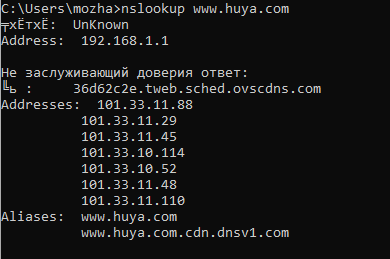
\includegraphics[scale=1]{screenshots/1.png}}
\label{fig:image}
\end{figure}

www.huya.com имеет несколько IP адресов \\
101.33.11.88 \\
101.33.11.29 \\
101.33.11.45 \\
101.33.10.114 \\
101.33.10.52 \\
101.33.11.48 \\
101.33.11.110 \\

\begin{figure}[h]
\center{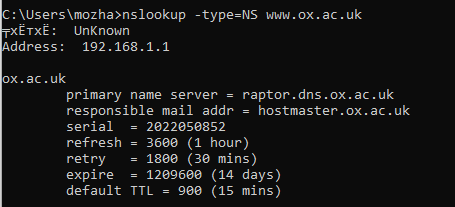
\includegraphics[scale=1]{screenshots/2.png}}
\label{fig:image}
\end{figure}

авторитетный DNS-сервер для Оксфорда raptor.dns.ox.ac.uk

\begin{figure}[h]
\center{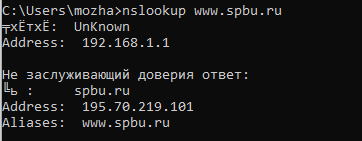
\includegraphics[scale=1]{screenshots/3.png}}
\label{fig:image}
\end{figure}

spbu.ru имеет один IP адрес 195.70.219.101
\newpage
2
\begin{figure}[h]
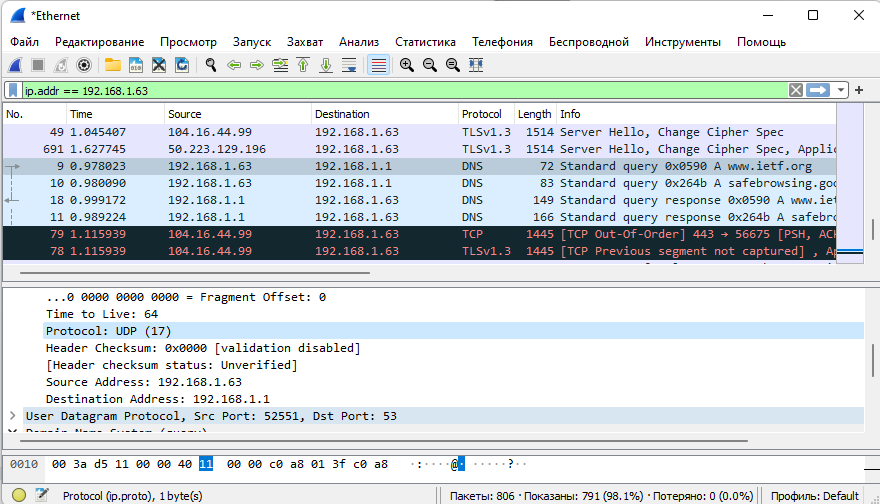
\includegraphics[width =\textwidth]{screenshots/4.png}
\label{fig:image}
\end{figure}

Протокол UDP, порт назначения 53

\begin{center}
\center{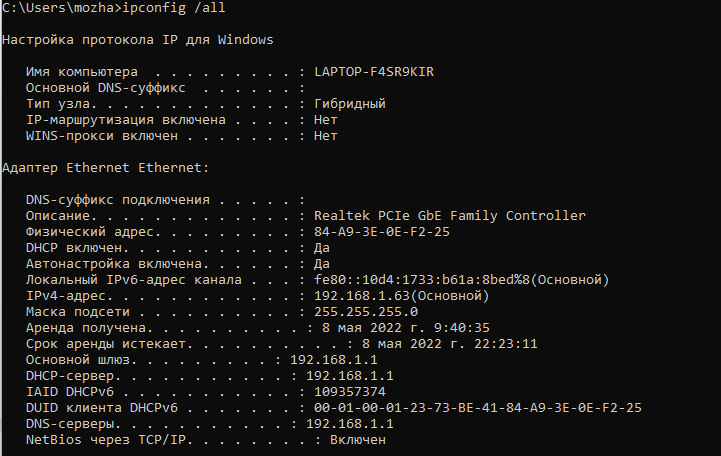
\includegraphics[width =\textwidth]{screenshots/5.png}}
\label{fig:image}
\end{center}

Отправлен на адрес 192.168.1.1, совпадает с локальным

\begin{center}
\center{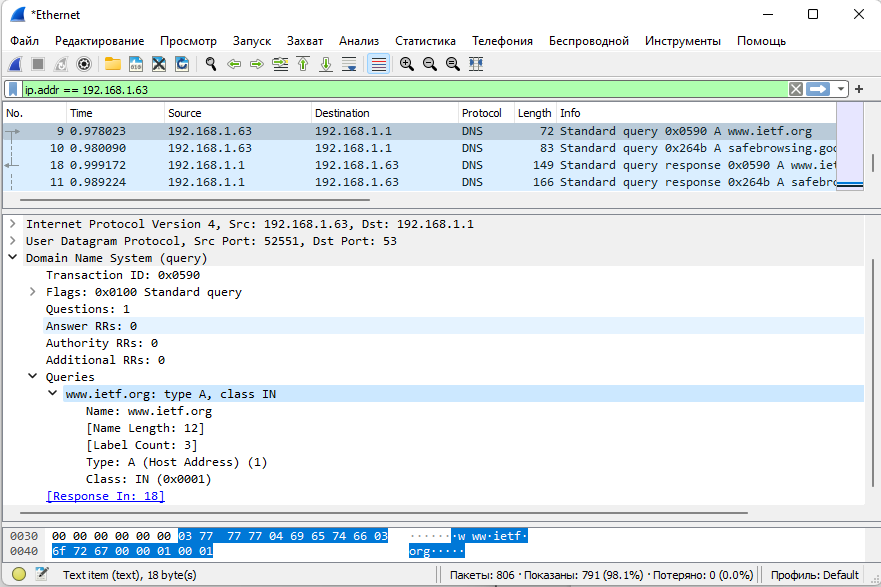
\includegraphics[width =\textwidth]{screenshots/6.png}}
\label{fig:image}
\end{center}

www.ietf.org: type A, class IN, ответов нет

\begin{center}
\center{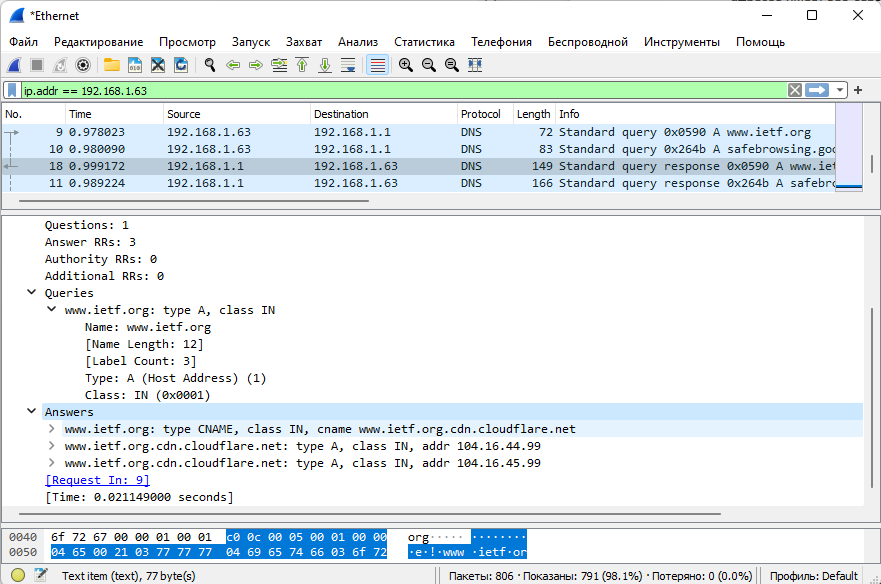
\includegraphics[width =\textwidth]{screenshots/7.png}}
\label{fig:image}
\end{center}

3 ответа, содержащие тип, класс, домен и адрес \\
www.ietf.org: type CNAME, class IN, cname www.ietf.org.cdn.cloudflare.net \\
www.ietf.org.cdn.cloudflare.net: type A, class IN, addr 104.16.44.99 \\
www.ietf.org.cdn.cloudflare.net: type A, class IN, addr 104.16.45.99 \\

\begin{center}
\center{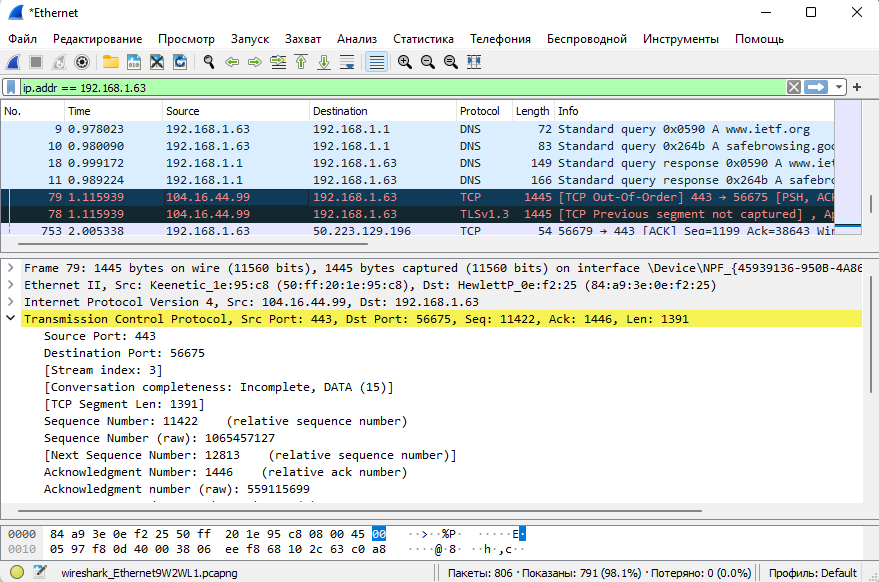
\includegraphics[width =\textwidth]{screenshots/8.png}}
\label{fig:image}
\end{center}
Адрес 104.16.44.99 совпадает,
новых DNS запросов не видно

\newpage
3
\begin{center}
\center{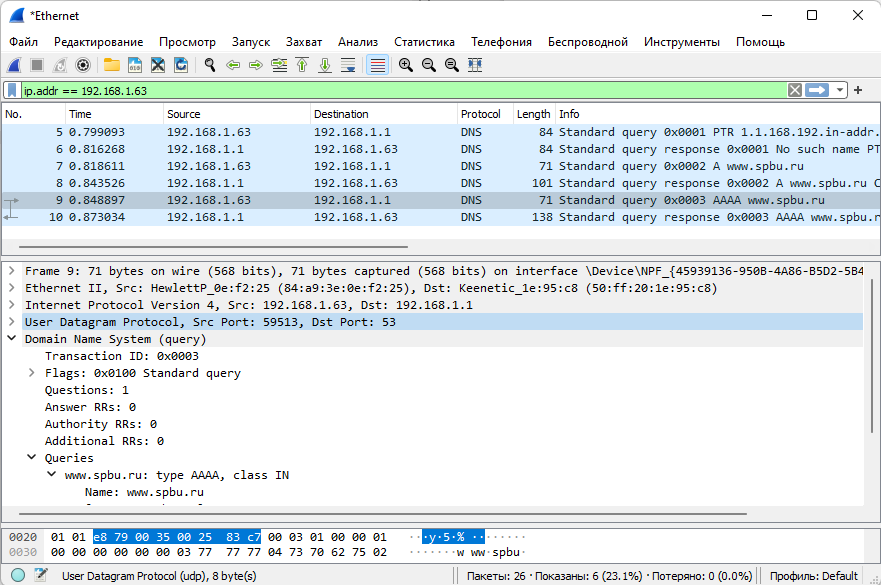
\includegraphics[width =\textwidth]{screenshots/9.png}}
\label{fig:image}
\end{center}
\begin{center}
\center{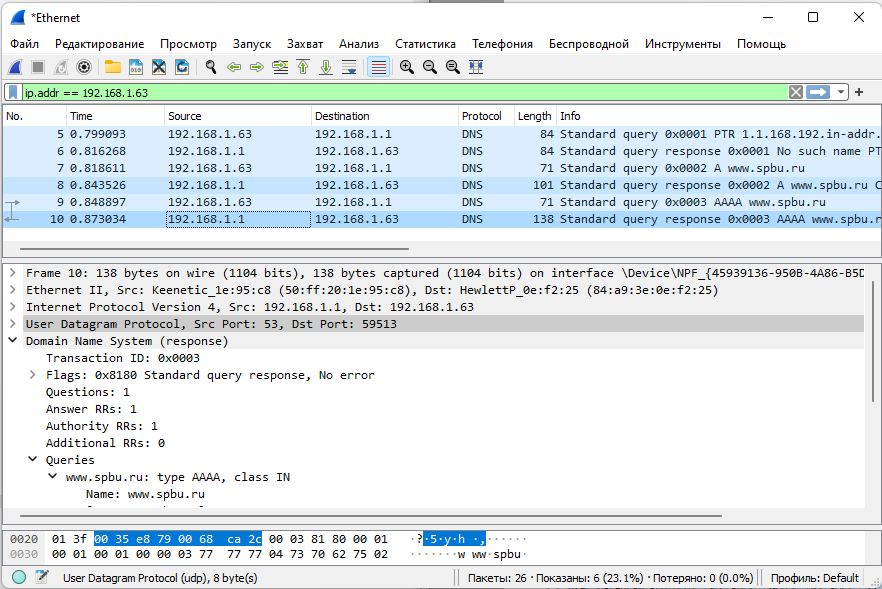
\includegraphics[width =\textwidth]{screenshots/10.png}}
\label{fig:image}
\end{center}

Порт 53 \\
Отправлен на адрес 192.168.1.1, совпадает с локальным 

\begin{center}
\center{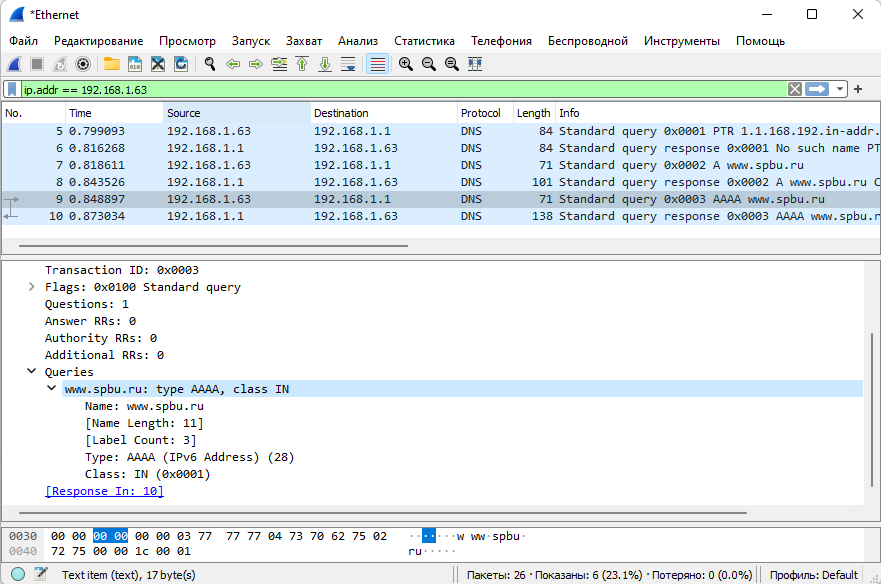
\includegraphics[width =\textwidth]{screenshots/11.png}}
\label{fig:image}
\end{center}

www.spbu.ru: type AAAA, class IN, ответов нет 

\begin{center}
\center{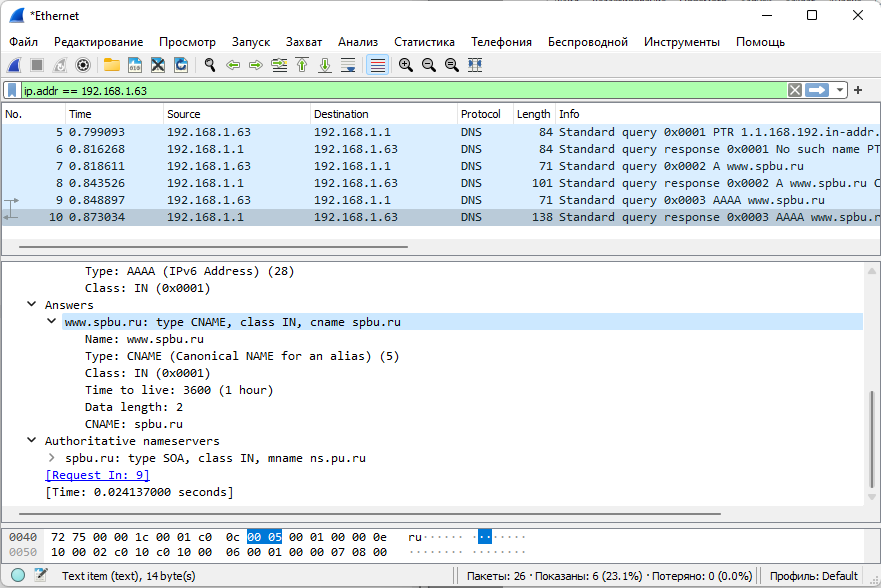
\includegraphics[width =\textwidth]{screenshots/12.png}}
\label{fig:image}
\end{center}

Ответ один: www.spbu.ru: type CNAME, class IN, cname spbu.ru

\newpage
4
\begin{center}
\center{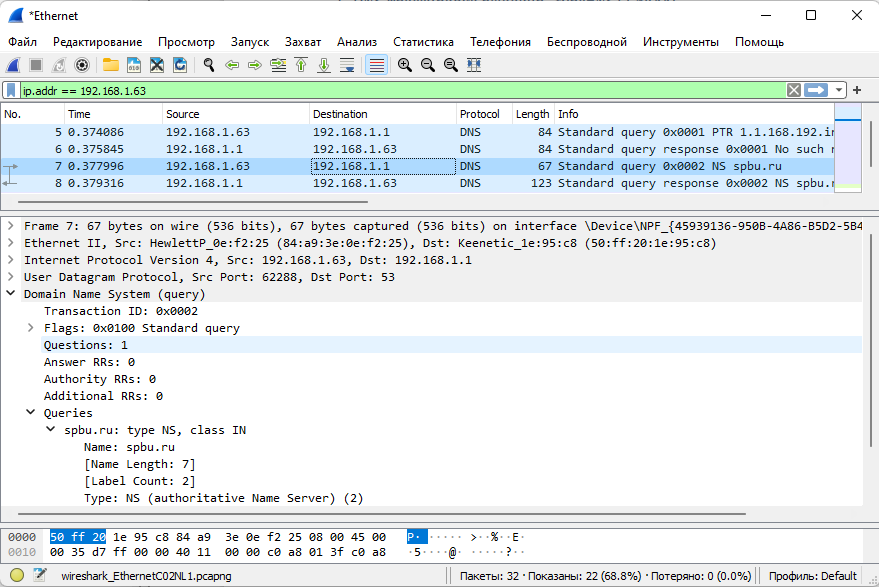
\includegraphics[width =\textwidth]{screenshots/13.png}}
\label{fig:image}
\end{center}
Отправлен на адрес 192.168.1.1, совпадает с локальным 

\begin{center}
\center{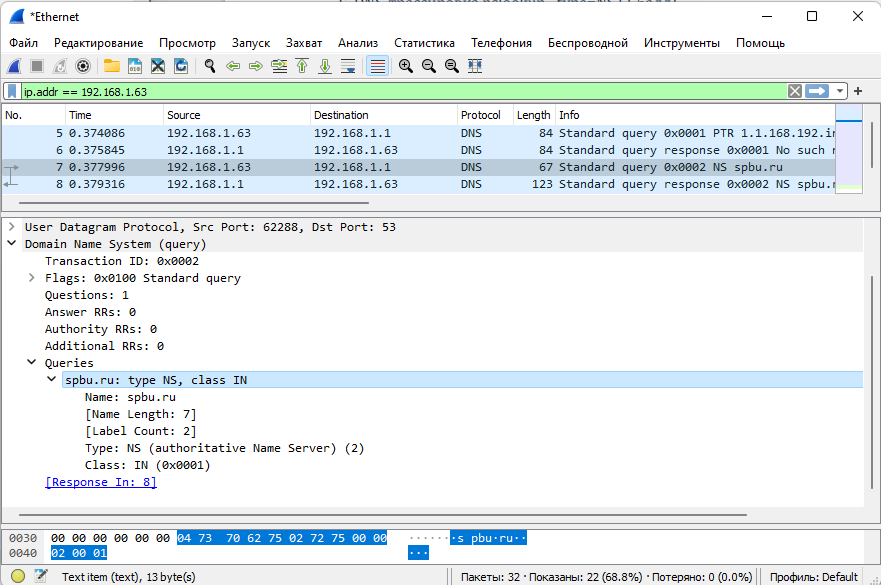
\includegraphics[width =\textwidth]{screenshots/14.png}}
\label{fig:image}
\end{center}
spbu.ru: type NS, class IN, ответов нет

\begin{center}
\center{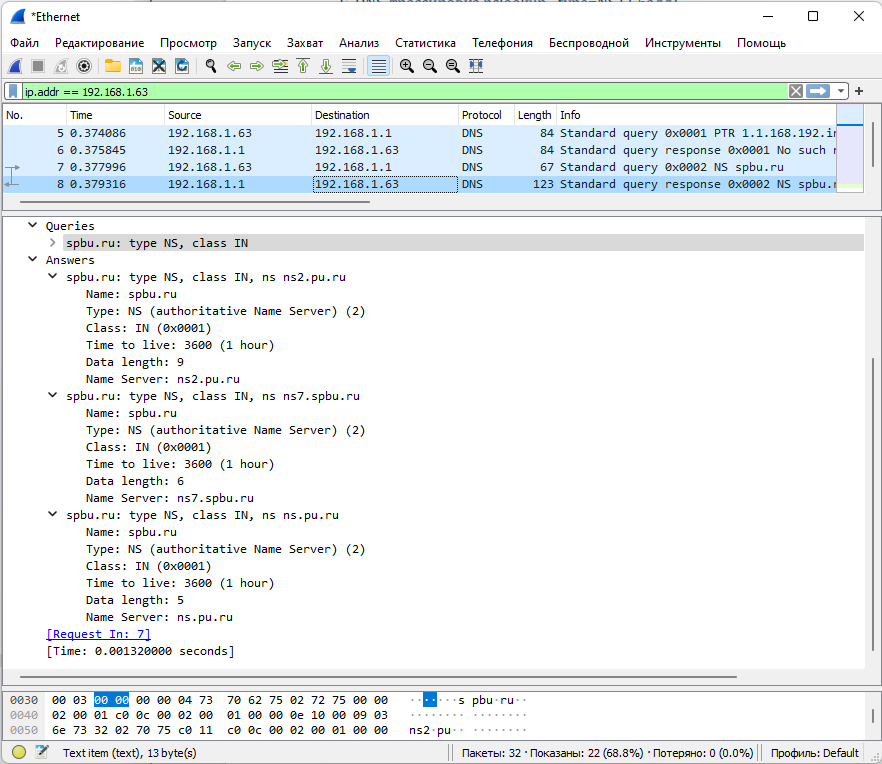
\includegraphics[width =\textwidth]{screenshots/15.png}}
\label{fig:image}
\end{center}
3 ответа, содержат тип, класс и имена ns серверов 

\newpage 
5
\begin{center}
\center{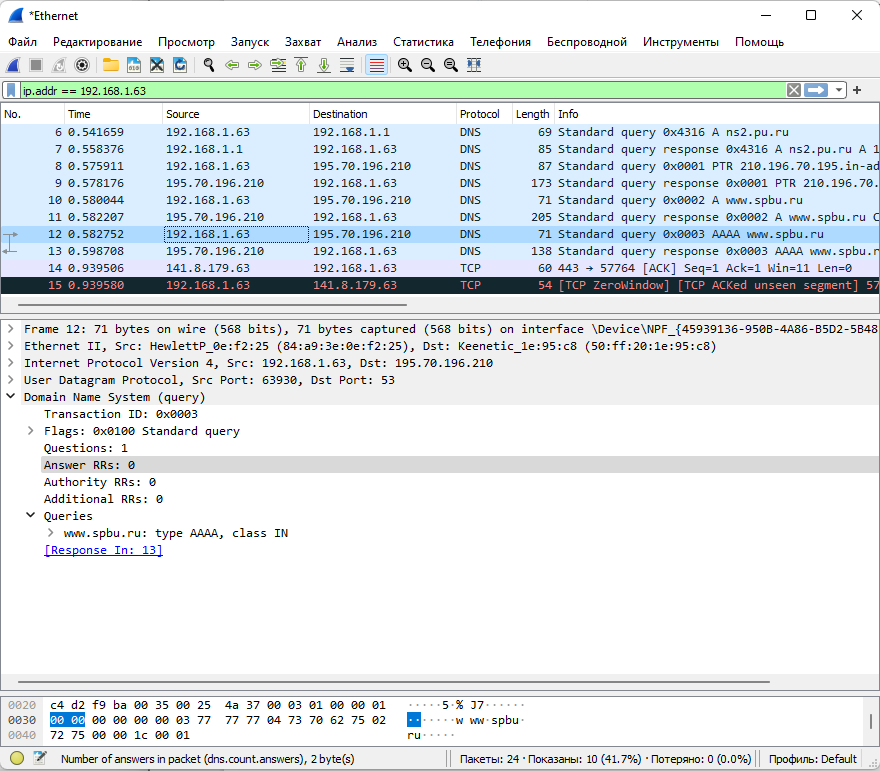
\includegraphics[width =\textwidth]{screenshots/16.png}}
\label{fig:image}
\end{center}
Адрес 195.70.196.210, это адрес ns2.pu.ru

\begin{center}
\center{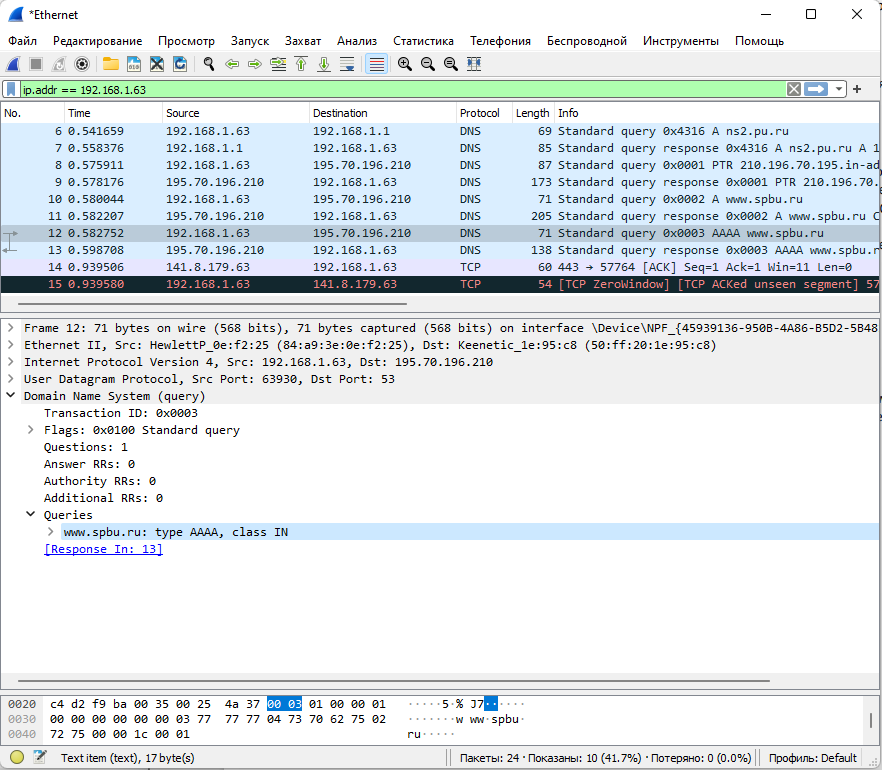
\includegraphics[width =\textwidth]{screenshots/17.png}}
\label{fig:image}
\end{center}
www.spbu.ru: type AAAA, class IN, ответов нет

\begin{center}
\center{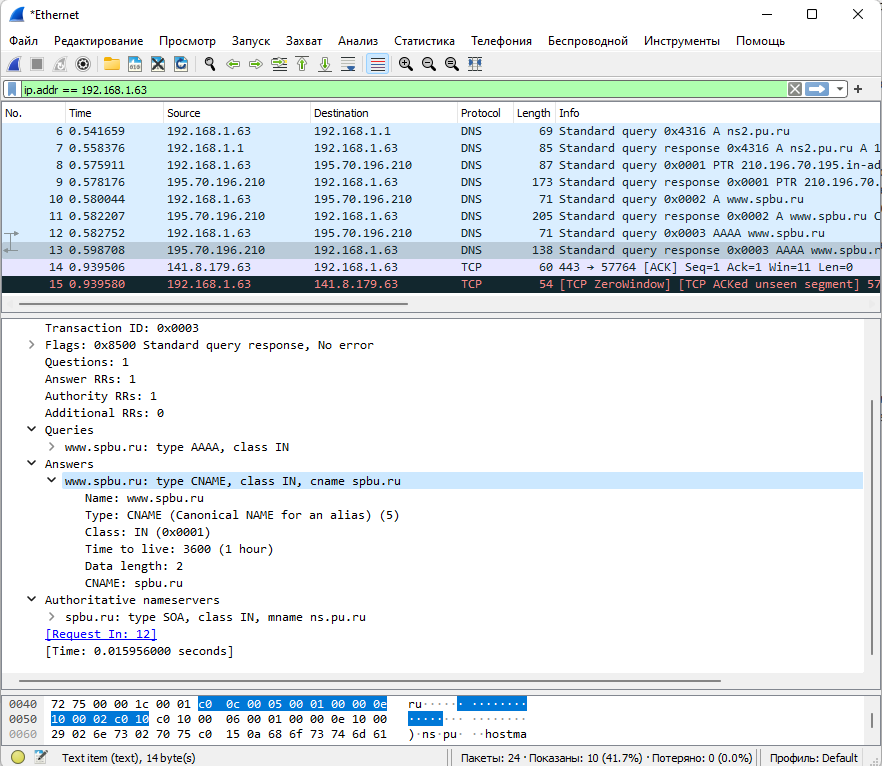
\includegraphics[width =\textwidth]{screenshots/18.png}}
\label{fig:image}
\end{center}
Ответ www.spbu.ru: type CNAME, class IN, cname spbu.ru

\newpage
6
whois - база данных со сведениями о доменах. Запись о домене обычно содержит имя и контактную информацию «регистранта» (владельца домена) и «регистратора» (организации, которая домен зарегистрировала), имена DNS серверов, дату регистрации и дату истечения срока ее действия. \\

https://2domains.ru/whois
\begin{center}
\center{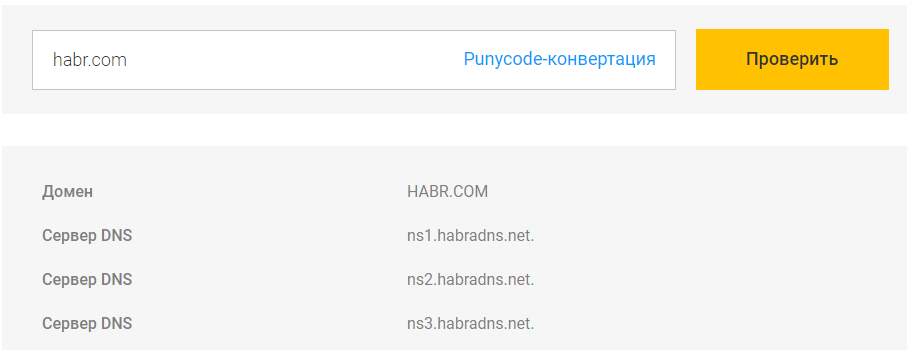
\includegraphics[width =\textwidth]{screenshots/19.png}}
\label{fig:image}
\end{center}

\begin{center}
\center{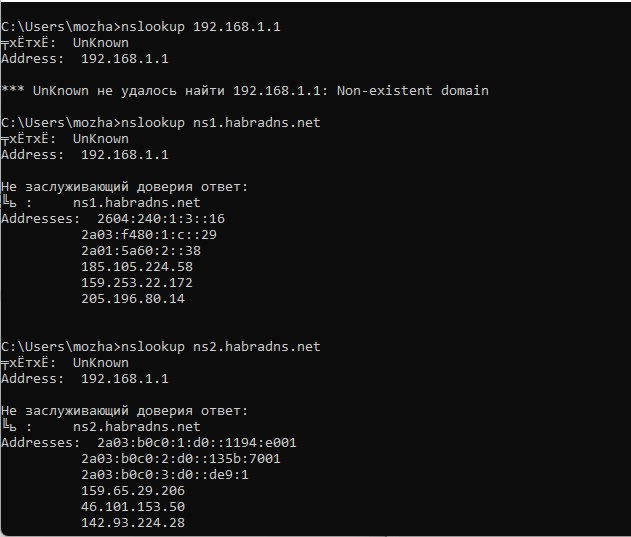
\includegraphics[width =\textwidth]{screenshots/20.png}}
\label{fig:image}
\end{center}
\end{document}








































